\documentclass[]{article}
\usepackage{lmodern}
\usepackage{amssymb,amsmath}
\usepackage{ifxetex,ifluatex}
\usepackage{fixltx2e} % provides \textsubscript
\ifnum 0\ifxetex 1\fi\ifluatex 1\fi=0 % if pdftex
  \usepackage[T1]{fontenc}
  \usepackage[utf8]{inputenc}
\else % if luatex or xelatex
  \ifxetex
    \usepackage{mathspec}
  \else
    \usepackage{fontspec}
  \fi
  \defaultfontfeatures{Ligatures=TeX,Scale=MatchLowercase}
\fi
% use upquote if available, for straight quotes in verbatim environments
\IfFileExists{upquote.sty}{\usepackage{upquote}}{}
% use microtype if available
\IfFileExists{microtype.sty}{%
\usepackage{microtype}
\UseMicrotypeSet[protrusion]{basicmath} % disable protrusion for tt fonts
}{}
\usepackage[margin=1in]{geometry}
\usepackage{hyperref}
\hypersetup{unicode=true,
            pdftitle={Tutorial 4: Linear Methods for Regression and Classification},
            pdfauthor={Introduction to Statistical Learning with Applications in R},
            pdfborder={0 0 0},
            breaklinks=true}
\urlstyle{same}  % don't use monospace font for urls
\usepackage{color}
\usepackage{fancyvrb}
\newcommand{\VerbBar}{|}
\newcommand{\VERB}{\Verb[commandchars=\\\{\}]}
\DefineVerbatimEnvironment{Highlighting}{Verbatim}{commandchars=\\\{\}}
% Add ',fontsize=\small' for more characters per line
\usepackage{framed}
\definecolor{shadecolor}{RGB}{248,248,248}
\newenvironment{Shaded}{\begin{snugshade}}{\end{snugshade}}
\newcommand{\KeywordTok}[1]{\textcolor[rgb]{0.13,0.29,0.53}{\textbf{#1}}}
\newcommand{\DataTypeTok}[1]{\textcolor[rgb]{0.13,0.29,0.53}{#1}}
\newcommand{\DecValTok}[1]{\textcolor[rgb]{0.00,0.00,0.81}{#1}}
\newcommand{\BaseNTok}[1]{\textcolor[rgb]{0.00,0.00,0.81}{#1}}
\newcommand{\FloatTok}[1]{\textcolor[rgb]{0.00,0.00,0.81}{#1}}
\newcommand{\ConstantTok}[1]{\textcolor[rgb]{0.00,0.00,0.00}{#1}}
\newcommand{\CharTok}[1]{\textcolor[rgb]{0.31,0.60,0.02}{#1}}
\newcommand{\SpecialCharTok}[1]{\textcolor[rgb]{0.00,0.00,0.00}{#1}}
\newcommand{\StringTok}[1]{\textcolor[rgb]{0.31,0.60,0.02}{#1}}
\newcommand{\VerbatimStringTok}[1]{\textcolor[rgb]{0.31,0.60,0.02}{#1}}
\newcommand{\SpecialStringTok}[1]{\textcolor[rgb]{0.31,0.60,0.02}{#1}}
\newcommand{\ImportTok}[1]{#1}
\newcommand{\CommentTok}[1]{\textcolor[rgb]{0.56,0.35,0.01}{\textit{#1}}}
\newcommand{\DocumentationTok}[1]{\textcolor[rgb]{0.56,0.35,0.01}{\textbf{\textit{#1}}}}
\newcommand{\AnnotationTok}[1]{\textcolor[rgb]{0.56,0.35,0.01}{\textbf{\textit{#1}}}}
\newcommand{\CommentVarTok}[1]{\textcolor[rgb]{0.56,0.35,0.01}{\textbf{\textit{#1}}}}
\newcommand{\OtherTok}[1]{\textcolor[rgb]{0.56,0.35,0.01}{#1}}
\newcommand{\FunctionTok}[1]{\textcolor[rgb]{0.00,0.00,0.00}{#1}}
\newcommand{\VariableTok}[1]{\textcolor[rgb]{0.00,0.00,0.00}{#1}}
\newcommand{\ControlFlowTok}[1]{\textcolor[rgb]{0.13,0.29,0.53}{\textbf{#1}}}
\newcommand{\OperatorTok}[1]{\textcolor[rgb]{0.81,0.36,0.00}{\textbf{#1}}}
\newcommand{\BuiltInTok}[1]{#1}
\newcommand{\ExtensionTok}[1]{#1}
\newcommand{\PreprocessorTok}[1]{\textcolor[rgb]{0.56,0.35,0.01}{\textit{#1}}}
\newcommand{\AttributeTok}[1]{\textcolor[rgb]{0.77,0.63,0.00}{#1}}
\newcommand{\RegionMarkerTok}[1]{#1}
\newcommand{\InformationTok}[1]{\textcolor[rgb]{0.56,0.35,0.01}{\textbf{\textit{#1}}}}
\newcommand{\WarningTok}[1]{\textcolor[rgb]{0.56,0.35,0.01}{\textbf{\textit{#1}}}}
\newcommand{\AlertTok}[1]{\textcolor[rgb]{0.94,0.16,0.16}{#1}}
\newcommand{\ErrorTok}[1]{\textcolor[rgb]{0.64,0.00,0.00}{\textbf{#1}}}
\newcommand{\NormalTok}[1]{#1}
\usepackage{graphicx,grffile}
\makeatletter
\def\maxwidth{\ifdim\Gin@nat@width>\linewidth\linewidth\else\Gin@nat@width\fi}
\def\maxheight{\ifdim\Gin@nat@height>\textheight\textheight\else\Gin@nat@height\fi}
\makeatother
% Scale images if necessary, so that they will not overflow the page
% margins by default, and it is still possible to overwrite the defaults
% using explicit options in \includegraphics[width, height, ...]{}
\setkeys{Gin}{width=\maxwidth,height=\maxheight,keepaspectratio}
\IfFileExists{parskip.sty}{%
\usepackage{parskip}
}{% else
\setlength{\parindent}{0pt}
\setlength{\parskip}{6pt plus 2pt minus 1pt}
}
\setlength{\emergencystretch}{3em}  % prevent overfull lines
\providecommand{\tightlist}{%
  \setlength{\itemsep}{0pt}\setlength{\parskip}{0pt}}
\setcounter{secnumdepth}{0}
% Redefines (sub)paragraphs to behave more like sections
\ifx\paragraph\undefined\else
\let\oldparagraph\paragraph
\renewcommand{\paragraph}[1]{\oldparagraph{#1}\mbox{}}
\fi
\ifx\subparagraph\undefined\else
\let\oldsubparagraph\subparagraph
\renewcommand{\subparagraph}[1]{\oldsubparagraph{#1}\mbox{}}
\fi

%%% Use protect on footnotes to avoid problems with footnotes in titles
\let\rmarkdownfootnote\footnote%
\def\footnote{\protect\rmarkdownfootnote}

%%% Change title format to be more compact
\usepackage{titling}

% Create subtitle command for use in maketitle
\newcommand{\subtitle}[1]{
  \posttitle{
    \begin{center}\large#1\end{center}
    }
}

\setlength{\droptitle}{-2em}

  \title{Tutorial 4: Linear Methods for Regression and Classification}
    \pretitle{\vspace{\droptitle}\centering\huge}
  \posttitle{\par}
    \author{Introduction to Statistical Learning with Applications in R}
    \preauthor{\centering\large\emph}
  \postauthor{\par}
    \date{}
    \predate{}\postdate{}
  

\begin{document}
\maketitle

This is an R Markdown document. Markdown is a simple formatting syntax
for authoring HTML, PDF, and MS Word documents. For more details on
using R Markdown see \url{http://rmarkdown.rstudio.com}.

\subsubsection{Simple Linear Regression}\label{simple-linear-regression}

In this example, we are going to use the dataset \texttt{state.x77} that
comes with standard \texttt{R} installation. It is a data set about the
50 states of united states.

Type \texttt{help(state.x77)} in your console window to read more about
this data set.

\begin{Shaded}
\begin{Highlighting}[]
\KeywordTok{library}\NormalTok{(datasets)}
\NormalTok{statedata=}\KeywordTok{as.data.frame}\NormalTok{(state.x77)}
\end{Highlighting}
\end{Shaded}

First we can modify the column names (the variable names) for easier
use. The function \texttt{colnames} can be used to retrieve the colume
names or assign new names.

\begin{Shaded}
\begin{Highlighting}[]
\KeywordTok{colnames}\NormalTok{(statedata)=}\KeywordTok{c}\NormalTok{(}\StringTok{"popu"}\NormalTok{, }\StringTok{"inc"}\NormalTok{, }\StringTok{"illit"}\NormalTok{, }\StringTok{"life.exp"}\NormalTok{, }\StringTok{"murder"}\NormalTok{, }\StringTok{"hs.grad"}\NormalTok{, }\StringTok{"frost"}\NormalTok{, }\StringTok{"area"}\NormalTok{)}
\end{Highlighting}
\end{Shaded}

\paragraph{Make a scatterplot.}\label{make-a-scatterplot.}

For this example, let's look at the association between life expectancy
(\texttt{life.exp}) and income (\texttt{inc}). The scatterplot below
shows a positive association between these two variables.

\begin{Shaded}
\begin{Highlighting}[]
\KeywordTok{plot}\NormalTok{(life.exp}\OperatorTok{~}\NormalTok{inc, }\DataTypeTok{data=}\NormalTok{statedata)}
\end{Highlighting}
\end{Shaded}

\includegraphics{Tutorial3_lineaer_methods_files/figure-latex/unnamed-chunk-3-1.pdf}

We can compute the correlation between these two variables. The value of
the correlation indicates a weak positive linear association.

\begin{Shaded}
\begin{Highlighting}[]
\KeywordTok{cor}\NormalTok{(statedata[,}\StringTok{"life.exp"}\NormalTok{], statedata[,}\StringTok{"inc"}\NormalTok{])}
\end{Highlighting}
\end{Shaded}

\begin{verbatim}
## [1] 0.3402553
\end{verbatim}

There is one observation that is far away from the rest of the points.
We would like to know which state is corresponding to that point. Let's
add state abbreviations to the plot.

\begin{Shaded}
\begin{Highlighting}[]
\KeywordTok{plot}\NormalTok{(life.exp}\OperatorTok{~}\NormalTok{inc, }\DataTypeTok{data=}\NormalTok{statedata, }\DataTypeTok{type=}\StringTok{"n"}\NormalTok{)}
\KeywordTok{text}\NormalTok{(life.exp}\OperatorTok{~}\NormalTok{inc, }\DataTypeTok{data=}\NormalTok{statedata, state.abb)}
\end{Highlighting}
\end{Shaded}

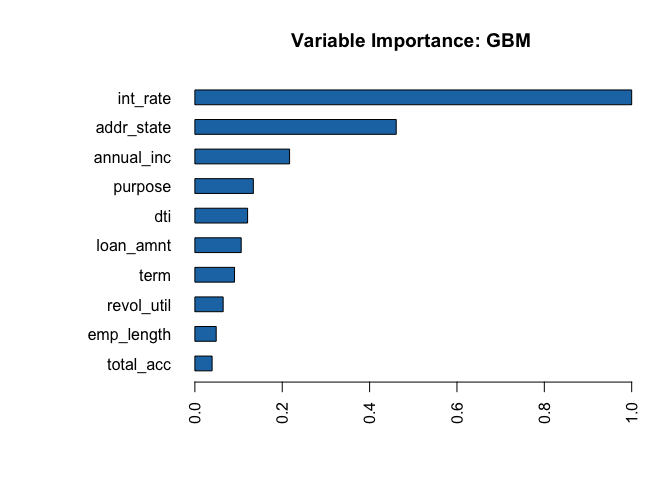
\includegraphics{Tutorial3_lineaer_methods_files/figure-latex/unnamed-chunk-5-1.pdf}

\paragraph{Fit a simple linear
regression}\label{fit-a-simple-linear-regression}

Now let's fit the following linear regression model between \(Y\)
(\texttt{life.exp}) and \(X\) (\texttt{inc})
\[ Y= \beta_0 +\beta_1 X + \varepsilon. \]

Here \(\beta_0\) and \(\beta_1\) are the regression coefficients of the
model and \(\varepsilon\) represents independent random errors.

Fitting a linear regression is to derive \[\hat{Y} = b_0 + b_1 X.\] Here
\(\hat{Y}\) is a fitted prediction for the observed life expectancies.
The difference \(Y - \hat{Y}\) is the prediction error, or residual.

\(b_0\) and \(b_1\) are estimates for the regression coefficients. They
are identified via the least square regression method that minimizes
\[\sum_{i=1}^n (Y - \hat{Y})^2,\] i.e., the sum of squared prediction
errors.

\begin{Shaded}
\begin{Highlighting}[]
\NormalTok{model1=}\KeywordTok{lm}\NormalTok{(life.exp}\OperatorTok{~}\NormalTok{inc, }\DataTypeTok{data=}\NormalTok{statedata)}
\KeywordTok{summary}\NormalTok{(model1)}
\end{Highlighting}
\end{Shaded}

\begin{verbatim}
## 
## Call:
## lm(formula = life.exp ~ inc, data = statedata)
## 
## Residuals:
##      Min       1Q   Median       3Q      Max 
## -2.96547 -0.76381 -0.03428  0.92876  2.32951 
## 
## Coefficients:
##              Estimate Std. Error t value Pr(>|t|)    
## (Intercept) 6.758e+01  1.328e+00  50.906   <2e-16 ***
## inc         7.433e-04  2.965e-04   2.507   0.0156 *  
## ---
## Signif. codes:  0 '***' 0.001 '**' 0.01 '*' 0.05 '.' 0.1 ' ' 1
## 
## Residual standard error: 1.275 on 48 degrees of freedom
## Multiple R-squared:  0.1158, Adjusted R-squared:  0.09735 
## F-statistic: 6.285 on 1 and 48 DF,  p-value: 0.01562
\end{verbatim}

In the above output, the intercept is \(b_0\) and the coeffient under
the column (\texttt{inc}) is \(b_1\)--the slope. The slope is estimated
to be \(7.4\times 10^{-4}\). The maganitude of this value does not mean
that the effect of income on life expectance is very small. This
maganitude is decided by the maganitude of the \(X\) variable and \(Y\)
variable.

\paragraph{Sampling uncertainty in regression
analysis}\label{sampling-uncertainty-in-regression-analysis}

Consider a population of 50 states and we identify the true regression
line in this population. Here the function \texttt{abline} add a
straight line to an existing plot.

\begin{Shaded}
\begin{Highlighting}[]
\KeywordTok{plot}\NormalTok{(life.exp}\OperatorTok{~}\NormalTok{inc, }\DataTypeTok{data=}\NormalTok{statedata,}
      \DataTypeTok{xlab=}\StringTok{"Life Expectancy"}\NormalTok{, }\DataTypeTok{ylab=}\StringTok{"Income"}\NormalTok{)}
\KeywordTok{abline}\NormalTok{(model1)}
\end{Highlighting}
\end{Shaded}

\includegraphics{Tutorial3_lineaer_methods_files/figure-latex/unnamed-chunk-7-1.pdf}

Now we can consider 4 random samples. We use a
\href{https://en.wikipedia.org/wiki/For_loop}{\texttt{for} loop} to run
an identical regression analysis on 4 randomly selected samples.

Within the loop, we will implement the following steps for each
repetition.

\begin{itemize}
\tightlist
\item
  Step 1: randomly select 10 states using the \texttt{sample} function
  of \texttt{R}.
\item
  Step 2: run least square regression on the selected states only
\item
  Step 3: compute a 95\% confidence band for the true regression line in
  the population using the sample.
\end{itemize}

\textbf{{[}Note{]}} The states are randomly selected in the following.
Therefore, every time you run this file, you will produce different
random samples that will give different estimated least regression
lines.

\begin{Shaded}
\begin{Highlighting}[]
\KeywordTok{par}\NormalTok{(}\DataTypeTok{mfrow=}\KeywordTok{c}\NormalTok{(}\DecValTok{2}\NormalTok{,}\DecValTok{2}\NormalTok{)) }\CommentTok{# create a panel of four plotting areas}

\ControlFlowTok{for}\NormalTok{(i }\ControlFlowTok{in} \DecValTok{1}\OperatorTok{:}\DecValTok{4}\NormalTok{)\{}
\NormalTok{  ## Plot the population}
  \KeywordTok{plot}\NormalTok{(life.exp}\OperatorTok{~}\NormalTok{inc, }\DataTypeTok{data=}\NormalTok{statedata,}
       \DataTypeTok{xlab=}\StringTok{"Life Expectancy"}\NormalTok{, }\DataTypeTok{ylab=}\StringTok{"Income"}\NormalTok{,}
       \DataTypeTok{title=}\KeywordTok{paste}\NormalTok{(}\StringTok{"Random sample"}\NormalTok{, }\KeywordTok{format}\NormalTok{(i)),}
       \DataTypeTok{ylim=}\KeywordTok{c}\NormalTok{(}\KeywordTok{min}\NormalTok{(life.exp), }\KeywordTok{max}\NormalTok{(life.exp)}\OperatorTok{+}\FloatTok{0.3}\NormalTok{))}
  \KeywordTok{abline}\NormalTok{(model1)}
  \ControlFlowTok{if}\NormalTok{(i}\OperatorTok{==}\DecValTok{1}\NormalTok{)\{}
    \KeywordTok{legend}\NormalTok{(}\DecValTok{3030}\NormalTok{, }\FloatTok{74.2}\NormalTok{, }
           \DataTypeTok{pch=}\KeywordTok{c}\NormalTok{(}\OtherTok{NA}\NormalTok{, }\OtherTok{NA}\NormalTok{, }\OtherTok{NA}\NormalTok{, }\DecValTok{1}\NormalTok{, }\DecValTok{16}\NormalTok{), }
           \DataTypeTok{lty=}\KeywordTok{c}\NormalTok{(}\DecValTok{1}\NormalTok{, }\DecValTok{1}\NormalTok{, }\DecValTok{2}\NormalTok{, }\OtherTok{NA}\NormalTok{, }\OtherTok{NA}\NormalTok{),}
           \DataTypeTok{col=}\KeywordTok{c}\NormalTok{(}\DecValTok{1}\NormalTok{, }\DecValTok{2}\NormalTok{, }\DecValTok{2}\NormalTok{, }\DecValTok{1}\NormalTok{, }\DecValTok{2}\NormalTok{),}
           \KeywordTok{c}\NormalTok{(}\StringTok{"population truth"}\NormalTok{, }\StringTok{"sample estimate"}\NormalTok{,}
             \StringTok{"sample confidence band"}\NormalTok{, }
             \StringTok{"states"}\NormalTok{, }\StringTok{"sampled"}\NormalTok{),}
           \DataTypeTok{cex=}\FloatTok{0.7}\NormalTok{,}
           \DataTypeTok{bty=}\StringTok{"n"}
\NormalTok{           )}
\NormalTok{  \}}
\NormalTok{  ## Select the sample}
\NormalTok{  selected.states=}\KeywordTok{sample}\NormalTok{(}\DecValTok{1}\OperatorTok{:}\DecValTok{50}\NormalTok{, }\DecValTok{10}\NormalTok{)}
  \KeywordTok{points}\NormalTok{(statedata[selected.states,}\StringTok{"inc"}\NormalTok{], }
\NormalTok{         statedata[selected.states,}\StringTok{"life.exp"}\NormalTok{], }\DataTypeTok{pch=}\DecValTok{16}\NormalTok{, }\DataTypeTok{col=}\DecValTok{2}\NormalTok{)}
\NormalTok{  ## Fit a regression line using the sample}
\NormalTok{  model.sel =}\StringTok{ }\KeywordTok{lm}\NormalTok{(life.exp}\OperatorTok{~}\NormalTok{inc, }\DataTypeTok{data=}\NormalTok{statedata[selected.states,])}
  \KeywordTok{abline}\NormalTok{(model.sel, }\DataTypeTok{col=}\DecValTok{2}\NormalTok{)}
\NormalTok{  ## Make a confidence band. }
\NormalTok{  #### first calculate the width of the band, W.}
\NormalTok{  ww=}\KeywordTok{qt}\NormalTok{(}\FloatTok{0.975}\NormalTok{, }\DecValTok{10}\OperatorTok{-}\DecValTok{2}\NormalTok{)}
\NormalTok{  #### generate plotting X values. }
\NormalTok{  plot.x<-}\KeywordTok{data.frame}\NormalTok{(}\DataTypeTok{inc=}\KeywordTok{seq}\NormalTok{(}\DecValTok{3000}\NormalTok{, }\DecValTok{7000}\NormalTok{, }\DecValTok{1}\NormalTok{))}
\NormalTok{  #### se.fit=T is an option to save }
\NormalTok{  #### the standard error of the fitted values. }
\NormalTok{  plot.fit<-}\KeywordTok{predict}\NormalTok{(model.sel, plot.x, }
                    \DataTypeTok{level=}\FloatTok{0.95}\NormalTok{, }\DataTypeTok{interval=}\StringTok{"confidence"}\NormalTok{, }
                    \DataTypeTok{se.fit=}\NormalTok{T)}

\NormalTok{  #### lines is a function to add connected lines }
\NormalTok{  #### to an existing plot.}
  \KeywordTok{lines}\NormalTok{(plot.x}\OperatorTok{$}\NormalTok{inc, plot.fit}\OperatorTok{$}\NormalTok{fit[,}\DecValTok{1}\NormalTok{]}\OperatorTok{+}\NormalTok{ww}\OperatorTok{*}\NormalTok{plot.fit}\OperatorTok{$}\NormalTok{se.fit, }
        \DataTypeTok{col=}\DecValTok{2}\NormalTok{, }\DataTypeTok{lty=}\DecValTok{2}\NormalTok{)}
  \KeywordTok{lines}\NormalTok{(plot.x}\OperatorTok{$}\NormalTok{inc, plot.fit}\OperatorTok{$}\NormalTok{fit[,}\DecValTok{1}\NormalTok{]}\OperatorTok{-}\NormalTok{ww}\OperatorTok{*}\NormalTok{plot.fit}\OperatorTok{$}\NormalTok{se.fit, }
        \DataTypeTok{col=}\DecValTok{2}\NormalTok{, }\DataTypeTok{lty=}\DecValTok{2}\NormalTok{)}
\NormalTok{\}}
\end{Highlighting}
\end{Shaded}

\begin{verbatim}
## Warning in plot.window(...): "title" is not a graphical parameter
\end{verbatim}

\begin{verbatim}
## Warning in plot.xy(xy, type, ...): "title" is not a graphical parameter
\end{verbatim}

\begin{verbatim}
## Warning in axis(side = side, at = at, labels = labels, ...): "title" is not
## a graphical parameter

## Warning in axis(side = side, at = at, labels = labels, ...): "title" is not
## a graphical parameter
\end{verbatim}

\begin{verbatim}
## Warning in box(...): "title" is not a graphical parameter
\end{verbatim}

\begin{verbatim}
## Warning in title(...): "title" is not a graphical parameter
\end{verbatim}

\begin{verbatim}
## Warning in plot.window(...): "title" is not a graphical parameter
\end{verbatim}

\begin{verbatim}
## Warning in plot.xy(xy, type, ...): "title" is not a graphical parameter
\end{verbatim}

\begin{verbatim}
## Warning in axis(side = side, at = at, labels = labels, ...): "title" is not
## a graphical parameter

## Warning in axis(side = side, at = at, labels = labels, ...): "title" is not
## a graphical parameter
\end{verbatim}

\begin{verbatim}
## Warning in box(...): "title" is not a graphical parameter
\end{verbatim}

\begin{verbatim}
## Warning in title(...): "title" is not a graphical parameter
\end{verbatim}

\begin{verbatim}
## Warning in plot.window(...): "title" is not a graphical parameter
\end{verbatim}

\begin{verbatim}
## Warning in plot.xy(xy, type, ...): "title" is not a graphical parameter
\end{verbatim}

\begin{verbatim}
## Warning in axis(side = side, at = at, labels = labels, ...): "title" is not
## a graphical parameter

## Warning in axis(side = side, at = at, labels = labels, ...): "title" is not
## a graphical parameter
\end{verbatim}

\begin{verbatim}
## Warning in box(...): "title" is not a graphical parameter
\end{verbatim}

\begin{verbatim}
## Warning in title(...): "title" is not a graphical parameter
\end{verbatim}

\begin{verbatim}
## Warning in plot.window(...): "title" is not a graphical parameter
\end{verbatim}

\begin{verbatim}
## Warning in plot.xy(xy, type, ...): "title" is not a graphical parameter
\end{verbatim}

\begin{verbatim}
## Warning in axis(side = side, at = at, labels = labels, ...): "title" is not
## a graphical parameter

## Warning in axis(side = side, at = at, labels = labels, ...): "title" is not
## a graphical parameter
\end{verbatim}

\begin{verbatim}
## Warning in box(...): "title" is not a graphical parameter
\end{verbatim}

\begin{verbatim}
## Warning in title(...): "title" is not a graphical parameter
\end{verbatim}

\includegraphics{Tutorial3_lineaer_methods_files/figure-latex/unnamed-chunk-8-1.pdf}

\subsubsection{Multiple Linear
Regression}\label{multiple-linear-regression}

The \texttt{MASS} library contains the \texttt{Boston} data set, which
records \texttt{medv} (median house value) for 506 neighborhoods around
Boston. We will seek to predict \texttt{medv} using 13 predictors such
as \texttt{rm} (average number of rooms per house), \texttt{age}
(average age of houses), and \texttt{lstat} (percent of households with
low socioeconomic status).

\begin{Shaded}
\begin{Highlighting}[]
\KeywordTok{library}\NormalTok{(MASS) }
\KeywordTok{library}\NormalTok{(ISLR)}
\end{Highlighting}
\end{Shaded}

In order to fit a multiple linear regression model using least squares,
we again use the \texttt{lm()} function. The syntax
\texttt{lm(y∼x1+x2+x3)} is used to fit a model with three predictors,
\texttt{x1}, \texttt{x2}, and \texttt{x3}. The \texttt{summary()}
function now outputs the regression coefficients for all the predictors.

\begin{Shaded}
\begin{Highlighting}[]
\KeywordTok{attach}\NormalTok{(Boston)}
\NormalTok{lm.fit=}\KeywordTok{lm}\NormalTok{(medv }\OperatorTok{~}\StringTok{ }\NormalTok{lstat}\OperatorTok{+}\NormalTok{age,}\DataTypeTok{data=}\NormalTok{Boston) }
\KeywordTok{summary}\NormalTok{(lm.fit)}
\end{Highlighting}
\end{Shaded}

\begin{verbatim}
## 
## Call:
## lm(formula = medv ~ lstat + age, data = Boston)
## 
## Residuals:
##     Min      1Q  Median      3Q     Max 
## -15.981  -3.978  -1.283   1.968  23.158 
## 
## Coefficients:
##             Estimate Std. Error t value Pr(>|t|)    
## (Intercept) 33.22276    0.73085  45.458  < 2e-16 ***
## lstat       -1.03207    0.04819 -21.416  < 2e-16 ***
## age          0.03454    0.01223   2.826  0.00491 ** 
## ---
## Signif. codes:  0 '***' 0.001 '**' 0.01 '*' 0.05 '.' 0.1 ' ' 1
## 
## Residual standard error: 6.173 on 503 degrees of freedom
## Multiple R-squared:  0.5513, Adjusted R-squared:  0.5495 
## F-statistic:   309 on 2 and 503 DF,  p-value: < 2.2e-16
\end{verbatim}

The Boston data set contains 13 variables, and so it would be cumbersome
to have to type all of these in order to perform a regression using all
of the predictors. Instead, we can use the following short-hand:

\begin{Shaded}
\begin{Highlighting}[]
\NormalTok{lm.fit=}\KeywordTok{lm}\NormalTok{(medv}\OperatorTok{~}\NormalTok{.,}\DataTypeTok{data=}\NormalTok{Boston) }
\KeywordTok{summary}\NormalTok{(lm.fit)}
\end{Highlighting}
\end{Shaded}

\begin{verbatim}
## 
## Call:
## lm(formula = medv ~ ., data = Boston)
## 
## Residuals:
##     Min      1Q  Median      3Q     Max 
## -15.595  -2.730  -0.518   1.777  26.199 
## 
## Coefficients:
##               Estimate Std. Error t value Pr(>|t|)    
## (Intercept)  3.646e+01  5.103e+00   7.144 3.28e-12 ***
## crim        -1.080e-01  3.286e-02  -3.287 0.001087 ** 
## zn           4.642e-02  1.373e-02   3.382 0.000778 ***
## indus        2.056e-02  6.150e-02   0.334 0.738288    
## chas         2.687e+00  8.616e-01   3.118 0.001925 ** 
## nox         -1.777e+01  3.820e+00  -4.651 4.25e-06 ***
## rm           3.810e+00  4.179e-01   9.116  < 2e-16 ***
## age          6.922e-04  1.321e-02   0.052 0.958229    
## dis         -1.476e+00  1.995e-01  -7.398 6.01e-13 ***
## rad          3.060e-01  6.635e-02   4.613 5.07e-06 ***
## tax         -1.233e-02  3.760e-03  -3.280 0.001112 ** 
## ptratio     -9.527e-01  1.308e-01  -7.283 1.31e-12 ***
## black        9.312e-03  2.686e-03   3.467 0.000573 ***
## lstat       -5.248e-01  5.072e-02 -10.347  < 2e-16 ***
## ---
## Signif. codes:  0 '***' 0.001 '**' 0.01 '*' 0.05 '.' 0.1 ' ' 1
## 
## Residual standard error: 4.745 on 492 degrees of freedom
## Multiple R-squared:  0.7406, Adjusted R-squared:  0.7338 
## F-statistic: 108.1 on 13 and 492 DF,  p-value: < 2.2e-16
\end{verbatim}

What if we would like to perform a regression using all of the variables
but one? For example, in the above regression output, \texttt{age} has a
high p-value. So we may wish to run a regression excluding this
predictor. The following syntax results in a regression using all
predictors except \texttt{age}.

\begin{Shaded}
\begin{Highlighting}[]
\NormalTok{lm.fit1=}\KeywordTok{lm}\NormalTok{(medv }\OperatorTok{~}\NormalTok{.}\OperatorTok{-}\NormalTok{age,}\DataTypeTok{data=}\NormalTok{Boston) }
\KeywordTok{summary}\NormalTok{(lm.fit1)}
\end{Highlighting}
\end{Shaded}

\begin{verbatim}
## 
## Call:
## lm(formula = medv ~ . - age, data = Boston)
## 
## Residuals:
##      Min       1Q   Median       3Q      Max 
## -15.6054  -2.7313  -0.5188   1.7601  26.2243 
## 
## Coefficients:
##               Estimate Std. Error t value Pr(>|t|)    
## (Intercept)  36.436927   5.080119   7.172 2.72e-12 ***
## crim         -0.108006   0.032832  -3.290 0.001075 ** 
## zn            0.046334   0.013613   3.404 0.000719 ***
## indus         0.020562   0.061433   0.335 0.737989    
## chas          2.689026   0.859598   3.128 0.001863 ** 
## nox         -17.713540   3.679308  -4.814 1.97e-06 ***
## rm            3.814394   0.408480   9.338  < 2e-16 ***
## dis          -1.478612   0.190611  -7.757 5.03e-14 ***
## rad           0.305786   0.066089   4.627 4.75e-06 ***
## tax          -0.012329   0.003755  -3.283 0.001099 ** 
## ptratio      -0.952211   0.130294  -7.308 1.10e-12 ***
## black         0.009321   0.002678   3.481 0.000544 ***
## lstat        -0.523852   0.047625 -10.999  < 2e-16 ***
## ---
## Signif. codes:  0 '***' 0.001 '**' 0.01 '*' 0.05 '.' 0.1 ' ' 1
## 
## Residual standard error: 4.74 on 493 degrees of freedom
## Multiple R-squared:  0.7406, Adjusted R-squared:  0.7343 
## F-statistic: 117.3 on 12 and 493 DF,  p-value: < 2.2e-16
\end{verbatim}

Alternatively, the \texttt{update()} function can be used.

\begin{Shaded}
\begin{Highlighting}[]
\NormalTok{lm.fit1=}\KeywordTok{lm}\NormalTok{(medv }\OperatorTok{~}\StringTok{ }\NormalTok{.}\OperatorTok{-}\NormalTok{age,}\DataTypeTok{data=}\NormalTok{Boston) }
\KeywordTok{summary}\NormalTok{(lm.fit1)}
\end{Highlighting}
\end{Shaded}

\begin{verbatim}
## 
## Call:
## lm(formula = medv ~ . - age, data = Boston)
## 
## Residuals:
##      Min       1Q   Median       3Q      Max 
## -15.6054  -2.7313  -0.5188   1.7601  26.2243 
## 
## Coefficients:
##               Estimate Std. Error t value Pr(>|t|)    
## (Intercept)  36.436927   5.080119   7.172 2.72e-12 ***
## crim         -0.108006   0.032832  -3.290 0.001075 ** 
## zn            0.046334   0.013613   3.404 0.000719 ***
## indus         0.020562   0.061433   0.335 0.737989    
## chas          2.689026   0.859598   3.128 0.001863 ** 
## nox         -17.713540   3.679308  -4.814 1.97e-06 ***
## rm            3.814394   0.408480   9.338  < 2e-16 ***
## dis          -1.478612   0.190611  -7.757 5.03e-14 ***
## rad           0.305786   0.066089   4.627 4.75e-06 ***
## tax          -0.012329   0.003755  -3.283 0.001099 ** 
## ptratio      -0.952211   0.130294  -7.308 1.10e-12 ***
## black         0.009321   0.002678   3.481 0.000544 ***
## lstat        -0.523852   0.047625 -10.999  < 2e-16 ***
## ---
## Signif. codes:  0 '***' 0.001 '**' 0.01 '*' 0.05 '.' 0.1 ' ' 1
## 
## Residual standard error: 4.74 on 493 degrees of freedom
## Multiple R-squared:  0.7406, Adjusted R-squared:  0.7343 
## F-statistic: 117.3 on 12 and 493 DF,  p-value: < 2.2e-16
\end{verbatim}

\subsubsection{Interaction Terms}\label{interaction-terms}

It is easy to include interaction terms in a linear model using the
\texttt{lm()} function. The syntax \texttt{lstat:black} tells \texttt{R}
to include an interaction term between \texttt{lstat} and
\texttt{black}. The syntax \texttt{lstat*age} simultaneously includes
\texttt{lstat}, \texttt{age}, and the interaction term lstat×age as
predictors; it is a shorthand for \texttt{lstat+age+lstat:age}.

\begin{Shaded}
\begin{Highlighting}[]
\KeywordTok{summary}\NormalTok{(}\KeywordTok{lm}\NormalTok{(medv }\OperatorTok{~}\StringTok{ }\NormalTok{lstat}\OperatorTok{*}\NormalTok{age,}\DataTypeTok{data=}\NormalTok{Boston))}
\end{Highlighting}
\end{Shaded}

\begin{verbatim}
## 
## Call:
## lm(formula = medv ~ lstat * age, data = Boston)
## 
## Residuals:
##     Min      1Q  Median      3Q     Max 
## -15.806  -4.045  -1.333   2.085  27.552 
## 
## Coefficients:
##               Estimate Std. Error t value Pr(>|t|)    
## (Intercept) 36.0885359  1.4698355  24.553  < 2e-16 ***
## lstat       -1.3921168  0.1674555  -8.313 8.78e-16 ***
## age         -0.0007209  0.0198792  -0.036   0.9711    
## lstat:age    0.0041560  0.0018518   2.244   0.0252 *  
## ---
## Signif. codes:  0 '***' 0.001 '**' 0.01 '*' 0.05 '.' 0.1 ' ' 1
## 
## Residual standard error: 6.149 on 502 degrees of freedom
## Multiple R-squared:  0.5557, Adjusted R-squared:  0.5531 
## F-statistic: 209.3 on 3 and 502 DF,  p-value: < 2.2e-16
\end{verbatim}

\subsubsection{Non-linear Transformations of the
Predictors}\label{non-linear-transformations-of-the-predictors}

\begin{Shaded}
\begin{Highlighting}[]
\KeywordTok{plot}\NormalTok{(lstat, medv, }\DataTypeTok{pch=}\DecValTok{16}\NormalTok{)}
\end{Highlighting}
\end{Shaded}

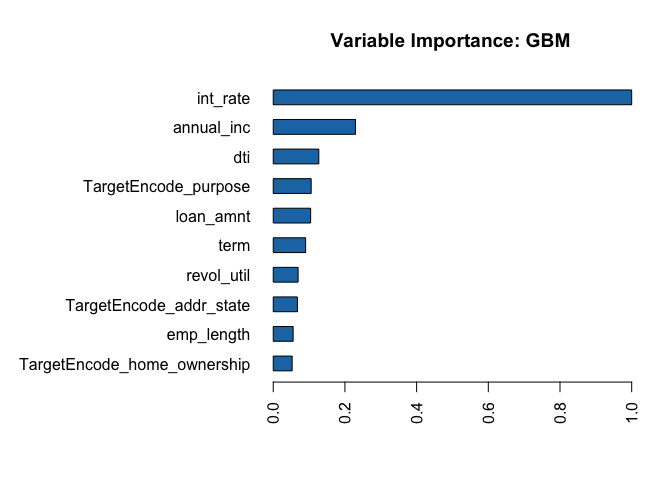
\includegraphics{Tutorial3_lineaer_methods_files/figure-latex/unnamed-chunk-15-1.pdf}

The \texttt{lm()} function can also accommodate non-linear
transformations of the predictors. For instance, given a predictor
\(X\), we can create a predictor \(X^2\) using \texttt{I(X\^{}2)}. The
function \texttt{I()} is needed since the \texttt{\^{}} has a special
meaning in a formula; wrapping as we do allows the standard usage in
\texttt{R}, which is \texttt{I()} to raise \texttt{X} to the power 2. We
now perform a regression of medv onto \texttt{lstat} and
\texttt{lstat}\(^2\).

\begin{Shaded}
\begin{Highlighting}[]
\NormalTok{lm.fit2=}\KeywordTok{lm}\NormalTok{(medv }\OperatorTok{~}\StringTok{ }\NormalTok{lstat}\OperatorTok{+}\KeywordTok{I}\NormalTok{(lstat}\OperatorTok{^}\DecValTok{2}\NormalTok{)) }
\KeywordTok{summary}\NormalTok{(lm.fit2)}
\end{Highlighting}
\end{Shaded}

\begin{verbatim}
## 
## Call:
## lm(formula = medv ~ lstat + I(lstat^2))
## 
## Residuals:
##      Min       1Q   Median       3Q      Max 
## -15.2834  -3.8313  -0.5295   2.3095  25.4148 
## 
## Coefficients:
##              Estimate Std. Error t value Pr(>|t|)    
## (Intercept) 42.862007   0.872084   49.15   <2e-16 ***
## lstat       -2.332821   0.123803  -18.84   <2e-16 ***
## I(lstat^2)   0.043547   0.003745   11.63   <2e-16 ***
## ---
## Signif. codes:  0 '***' 0.001 '**' 0.01 '*' 0.05 '.' 0.1 ' ' 1
## 
## Residual standard error: 5.524 on 503 degrees of freedom
## Multiple R-squared:  0.6407, Adjusted R-squared:  0.6393 
## F-statistic: 448.5 on 2 and 503 DF,  p-value: < 2.2e-16
\end{verbatim}

The near-zero p-value associated with the quadratic term suggests that
it leads to an improved model. We use the \texttt{anova()} function to
further quantify the extent to which the quadratic fit is superior to
the linear fit.

\begin{Shaded}
\begin{Highlighting}[]
\NormalTok{lm.fit=}\KeywordTok{lm}\NormalTok{(medv}\OperatorTok{~}\NormalTok{lstat) }
\KeywordTok{anova}\NormalTok{(lm.fit ,lm.fit2)}
\end{Highlighting}
\end{Shaded}

\begin{verbatim}
## Analysis of Variance Table
## 
## Model 1: medv ~ lstat
## Model 2: medv ~ lstat + I(lstat^2)
##   Res.Df   RSS Df Sum of Sq     F    Pr(>F)    
## 1    504 19472                                 
## 2    503 15347  1    4125.1 135.2 < 2.2e-16 ***
## ---
## Signif. codes:  0 '***' 0.001 '**' 0.01 '*' 0.05 '.' 0.1 ' ' 1
\end{verbatim}

Here Model 1 represents the linear submodel containing only one
predictor, \texttt{lstat}, while Model 2 corresponds to the larger
quadratic model that has two predictors, \texttt{lstat} and
\texttt{lstat}\(^2\). The \texttt{anova()} function performs a
hypothesis test comparing the two models. The null hypothesis is that
the two models fit the data equally well, and the alternative hypothesis
is that the full model is superior. Here the F-statistic is 135 and the
associated p-value is virtually zero. This provides very clear evidence
that the model containing the predictors \texttt{lstat} and
\texttt{lstat}\(^2\) is far superior to the model that only contains the
predictor lstat. This is not surprising, since earlier we saw evidence
for non-linearity in the relationship between \texttt{medv} and
\texttt{lstat}. If we type

\begin{Shaded}
\begin{Highlighting}[]
\KeywordTok{par}\NormalTok{(}\DataTypeTok{mfrow=}\KeywordTok{c}\NormalTok{(}\DecValTok{2}\NormalTok{,}\DecValTok{2}\NormalTok{)) }
\KeywordTok{plot}\NormalTok{(lm.fit2)}
\end{Highlighting}
\end{Shaded}

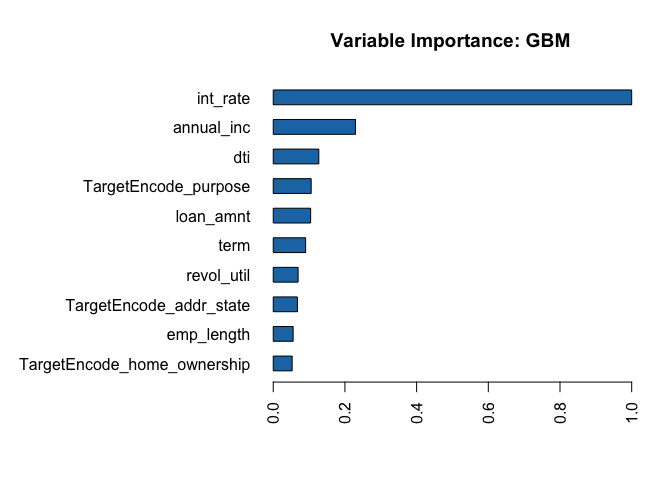
\includegraphics{Tutorial3_lineaer_methods_files/figure-latex/unnamed-chunk-18-1.pdf}

then we see that when the \texttt{lstat}\(^2\) term is included in the
model, there is little discernible pattern in the residuals.

\subsubsection{Qualitative Predictors}\label{qualitative-predictors}

We will now examine the \texttt{Carseats} data, which is part of the
\texttt{ISLR} library. We will attempt to predict \texttt{Sales} (child
car seat sales) in 400 locations based on a number of predictors.

\begin{Shaded}
\begin{Highlighting}[]
\KeywordTok{names}\NormalTok{(Carseats )}
\end{Highlighting}
\end{Shaded}

\begin{verbatim}
##  [1] "Sales"       "CompPrice"   "Income"      "Advertising" "Population" 
##  [6] "Price"       "ShelveLoc"   "Age"         "Education"   "Urban"      
## [11] "US"
\end{verbatim}

The \texttt{Carseats} data includes qualitative predictors such as
\texttt{Shelveloc}, an in- dicator of the quality of the shelving
location—that is, the space within a store in which the car seat is
displayed—at each location. The predictor \texttt{Shelveloc} takes on
three possible values, \emph{Bad}, \emph{Medium}, and \emph{Good}.

Given a qualitative variable such as \texttt{Shelveloc}, \texttt{R}
generates dummy variables automatically. Below we fit a multiple
regression model that includes some interaction terms.

\begin{Shaded}
\begin{Highlighting}[]
\NormalTok{lm.fit=}\KeywordTok{lm}\NormalTok{(Sales}\OperatorTok{~}\NormalTok{.}\OperatorTok{+}\NormalTok{Income}\OperatorTok{:}\NormalTok{Advertising}\OperatorTok{+}\NormalTok{Price}\OperatorTok{:}\NormalTok{Age,}\DataTypeTok{data=}\NormalTok{Carseats)}
\KeywordTok{summary}\NormalTok{(lm.fit)}
\end{Highlighting}
\end{Shaded}

\begin{verbatim}
## 
## Call:
## lm(formula = Sales ~ . + Income:Advertising + Price:Age, data = Carseats)
## 
## Residuals:
##     Min      1Q  Median      3Q     Max 
## -2.9208 -0.7503  0.0177  0.6754  3.3413 
## 
## Coefficients:
##                      Estimate Std. Error t value Pr(>|t|)    
## (Intercept)         6.5755654  1.0087470   6.519 2.22e-10 ***
## CompPrice           0.0929371  0.0041183  22.567  < 2e-16 ***
## Income              0.0108940  0.0026044   4.183 3.57e-05 ***
## Advertising         0.0702462  0.0226091   3.107 0.002030 ** 
## Population          0.0001592  0.0003679   0.433 0.665330    
## Price              -0.1008064  0.0074399 -13.549  < 2e-16 ***
## ShelveLocGood       4.8486762  0.1528378  31.724  < 2e-16 ***
## ShelveLocMedium     1.9532620  0.1257682  15.531  < 2e-16 ***
## Age                -0.0579466  0.0159506  -3.633 0.000318 ***
## Education          -0.0208525  0.0196131  -1.063 0.288361    
## UrbanYes            0.1401597  0.1124019   1.247 0.213171    
## USYes              -0.1575571  0.1489234  -1.058 0.290729    
## Income:Advertising  0.0007510  0.0002784   2.698 0.007290 ** 
## Price:Age           0.0001068  0.0001333   0.801 0.423812    
## ---
## Signif. codes:  0 '***' 0.001 '**' 0.01 '*' 0.05 '.' 0.1 ' ' 1
## 
## Residual standard error: 1.011 on 386 degrees of freedom
## Multiple R-squared:  0.8761, Adjusted R-squared:  0.8719 
## F-statistic:   210 on 13 and 386 DF,  p-value: < 2.2e-16
\end{verbatim}

The \texttt{contrasts()} function returns the coding that \texttt{R}
uses for the dummy variables.

\begin{Shaded}
\begin{Highlighting}[]
\KeywordTok{attach}\NormalTok{(Carseats)}
\KeywordTok{contrasts}\NormalTok{(ShelveLoc)}
\end{Highlighting}
\end{Shaded}

\begin{verbatim}
##        Good Medium
## Bad       0      0
## Good      1      0
## Medium    0      1
\end{verbatim}

\texttt{R} has created a \texttt{ShelveLocGood} dummy variable that
takes on a value of 1 if the shelving location is good, and 0 otherwise.
It has also created a \texttt{ShelveLocMedium} dummy variable that
equals 1 if the shelving location is medium, and 0 otherwise. A bad
shelving location corresponds to a zero for each of the two dummy
variables. The fact that the coefficient for \texttt{ShelveLocGood} in
the regression output is positive indicates that a good shelving
location is associated with high sales (relative to a bad location). And
\texttt{ShelveLocMedium} has a smaller positive coefficient, indicating
that a medium shelving location leads to higher sales than a bad
shelving location but lower sales than a good shelving location.

\subsubsection{Logistic Regression}\label{logistic-regression}

This part, we focus on a classification problem. We will apply logistic
regression to the iris data. First, we download the data

\begin{Shaded}
\begin{Highlighting}[]
\NormalTok{iris =}\StringTok{ }\KeywordTok{read.table}\NormalTok{(}\StringTok{"http://archive.ics.uci.edu/ml/machine-learning-databases/iris/iris.data"}\NormalTok{, }\DataTypeTok{sep =} \StringTok{","}\NormalTok{, }\DataTypeTok{header =} \OtherTok{FALSE}\NormalTok{)}
\KeywordTok{names}\NormalTok{(iris) =}\StringTok{ }\KeywordTok{c}\NormalTok{(}\StringTok{"sepal.length"}\NormalTok{, }\StringTok{"sepal.width"}\NormalTok{, }\StringTok{"petal.length"}\NormalTok{, }\StringTok{"petal.width"}\NormalTok{, }\StringTok{"iris.type"}\NormalTok{)}
\NormalTok{### attach name to each column so that we can directly access each column by its name}
\KeywordTok{attach}\NormalTok{(iris)}
\end{Highlighting}
\end{Shaded}

We randomly split the data into training set and test set.

\begin{Shaded}
\begin{Highlighting}[]
\NormalTok{train =}\StringTok{ }\KeywordTok{sample.int}\NormalTok{(}\KeywordTok{nrow}\NormalTok{(iris), }\DecValTok{100}\NormalTok{)}
\end{Highlighting}
\end{Shaded}

The \texttt{glm()} function in \texttt{R} can only deal with binary
classification problems. Let’s try to distinguish Setosa apart from
Virginica, Versicolor.

\begin{Shaded}
\begin{Highlighting}[]
\NormalTok{Y =}\StringTok{ }\NormalTok{iris.type }\OperatorTok{==}\StringTok{ "Iris-setosa"}
\NormalTok{logistic.model =}\StringTok{ }\KeywordTok{glm}\NormalTok{(Y }\OperatorTok{~}\StringTok{ }\NormalTok{sepal.length }\OperatorTok{+}\StringTok{ }\NormalTok{sepal.width, }\DataTypeTok{data=}\NormalTok{iris, }\DataTypeTok{family =} \KeywordTok{binomial}\NormalTok{(), }\DataTypeTok{subset=}\NormalTok{train)}
\end{Highlighting}
\end{Shaded}

\begin{verbatim}
## Warning: glm.fit: algorithm did not converge
\end{verbatim}

\begin{verbatim}
## Warning: glm.fit: fitted probabilities numerically 0 or 1 occurred
\end{verbatim}

\begin{Shaded}
\begin{Highlighting}[]
\NormalTok{logistic.model}
\end{Highlighting}
\end{Shaded}

\begin{verbatim}
## 
## Call:  glm(formula = Y ~ sepal.length + sepal.width, family = binomial(), 
##     data = iris, subset = train)
## 
## Coefficients:
##  (Intercept)  sepal.length   sepal.width  
##        445.7        -166.7         140.9  
## 
## Degrees of Freedom: 99 Total (i.e. Null);  97 Residual
## Null Deviance:       114.6 
## Residual Deviance: 1.857e-08     AIC: 6
\end{verbatim}

We can visualize the model in a two-dimensional plot.

\begin{Shaded}
\begin{Highlighting}[]
\KeywordTok{plot}\NormalTok{(sepal.length[train], sepal.width[train], }\DataTypeTok{type=}\StringTok{'p'}\NormalTok{,}\DataTypeTok{pch=}\DecValTok{16}\NormalTok{, }\DataTypeTok{col=}\NormalTok{(Y[train]}\OperatorTok{+}\DecValTok{4}\NormalTok{), }\DataTypeTok{xlab=}\StringTok{"Sepal Length"}\NormalTok{, }\DataTypeTok{ylab=}\StringTok{"Sepal Width"}\NormalTok{)}
\KeywordTok{abline}\NormalTok{(}\DataTypeTok{a =} \OperatorTok{-}\NormalTok{logistic.model}\OperatorTok{$}\NormalTok{coefficients[}\DecValTok{1}\NormalTok{]}\OperatorTok{/}\NormalTok{logistic.model}\OperatorTok{$}\NormalTok{coefficients[}\DecValTok{3}\NormalTok{], }\DataTypeTok{b =} \OperatorTok{-}\NormalTok{logistic.model}\OperatorTok{$}\NormalTok{coefficients[}\DecValTok{2}\NormalTok{]}\OperatorTok{/}\NormalTok{logistic.model}\OperatorTok{$}\NormalTok{coefficients[}\DecValTok{3}\NormalTok{], }\DataTypeTok{col=}\StringTok{'gray'}\NormalTok{, }\DataTypeTok{lwd=}\DecValTok{2}\NormalTok{)}
\end{Highlighting}
\end{Shaded}

\includegraphics{Tutorial3_lineaer_methods_files/figure-latex/unnamed-chunk-25-1.pdf}

To make predictions on the test set, we call the function
\texttt{predict()}

\begin{Shaded}
\begin{Highlighting}[]
\NormalTok{glm.probs =}\StringTok{ }\KeywordTok{predict}\NormalTok{(logistic.model, iris[}\OperatorTok{-}\NormalTok{train,], }\DataTypeTok{type=}\StringTok{"response"}\NormalTok{)}
\NormalTok{glm.pred =}\StringTok{ }\NormalTok{glm.probs}\OperatorTok{>}\FloatTok{0.5}
\NormalTok{### summrize the prediction by a confusion matrix}
\KeywordTok{table}\NormalTok{(Y[}\OperatorTok{-}\NormalTok{train], glm.pred)}
\end{Highlighting}
\end{Shaded}

\begin{verbatim}
##        glm.pred
##         FALSE TRUE
##   FALSE    26    0
##   TRUE      0   24
\end{verbatim}

\subsubsection{Linear Discriminant
Analysis}\label{linear-discriminant-analysis}

We can also perfom LDA on the same data set. In \texttt{R}, we fit a LDA
model using the \texttt{lda()} function, which is part of the
\texttt{MASS} library.

\begin{Shaded}
\begin{Highlighting}[]
\KeywordTok{library}\NormalTok{(MASS)}
\NormalTok{lda.model<-}\KeywordTok{lda}\NormalTok{(Y }\OperatorTok{~}\StringTok{ }\NormalTok{sepal.length }\OperatorTok{+}\StringTok{ }\NormalTok{sepal.width, }\DataTypeTok{data=}\NormalTok{iris, }\DataTypeTok{subset=}\NormalTok{train)}
\NormalTok{lda.model}
\end{Highlighting}
\end{Shaded}

\begin{verbatim}
## Call:
## lda(Y ~ sepal.length + sepal.width, data = iris, subset = train)
## 
## Prior probabilities of groups:
## FALSE  TRUE 
##  0.74  0.26 
## 
## Group means:
##       sepal.length sepal.width
## FALSE     6.224324    2.856757
## TRUE      5.003846    3.419231
## 
## Coefficients of linear discriminants:
##                    LD1
## sepal.length -1.854788
## sepal.width   2.798932
\end{verbatim}

\begin{Shaded}
\begin{Highlighting}[]
\KeywordTok{plot}\NormalTok{(lda.model)}
\end{Highlighting}
\end{Shaded}

\includegraphics{Tutorial3_lineaer_methods_files/figure-latex/unnamed-chunk-27-1.pdf}

To make predictions, we call the function \texttt{predict()}

\begin{Shaded}
\begin{Highlighting}[]
\NormalTok{lda.pred =}\StringTok{ }\KeywordTok{predict}\NormalTok{(lda.model, iris[}\OperatorTok{-}\NormalTok{train,])}
\KeywordTok{table}\NormalTok{(Y[}\OperatorTok{-}\NormalTok{train], lda.pred}\OperatorTok{$}\NormalTok{class)}
\end{Highlighting}
\end{Shaded}

\begin{verbatim}
##        
##         FALSE TRUE
##   FALSE    26    0
##   TRUE      0   24
\end{verbatim}

For this data set, the LDA and logistic regression predictions are
almost identical.


\end{document}
